\documentclass[12pt]{article}
\usepackage{amsmath}
\usepackage{amssymb}
\usepackage{listings}
\usepackage{titling}
\usepackage{fancyhdr}
\usepackage{sectsty}
\usepackage{titlesec}
\usepackage{xcolor}
\usepackage{enumitem}
\usepackage{array}
\usepackage{comment}
\usepackage[utf8]{inputenc}
\usepackage{amsmath,amssymb,graphicx,url,mathrsfs}
\usepackage{float}
\usepackage[pdftex,pdfpagelabels,bookmarks,hyperindex,hyperfigures]{hyperref}
\usepackage{import}
\usepackage{caption}
\usepackage[paperwidth=21cm, paperheight=29.7cm, top=2.5cm, bottom=2.5cm, left=2.5cm, right=2.5cm]{geometry}
\fancyhf{}
\rfoot{\thepage}
\renewcommand{\headrulewidth}{0pt}

\definecolor{commentgreen}{RGB}{28,172,0}
\lstset{language=python, breaklines=true, basicstyle=\ttfamily, commentstyle=\color{commentgreen}, keywordstyle=\color{blue}, morekeywords = {True, False}, identifierstyle=\color{black}, showstringspaces=false}

\begin{document}
%
%\thispagestyle{fancy}
%\pagestyle{fancy}
%
\pagenumbering{gobble}
\vspace*{\fill}
\begin{center}
\Huge{37}\huge{ IN }\Huge{1}\huge{ }\Huge{S}\huge{ENSOR }\Huge{K}\huge{IT}
\end{center}
\begin{center}
\Large{ESP32}\normalsize{ \& }\Large{M}\normalsize{ICRO}\Large{P}\normalsize{YTHON }\large{R}\normalsize{EFERENCE}
\end{center}
\vspace*{\fill}

\newpage
\tableofcontents
%\listoffigures
%\listoftables
\lstlistoflistings

\newpage
\pagestyle{fancy}
\pagenumbering{arabic}

\begin{comment}
\section{ESP32 \& MicroPython}

\begin{figure}[H]
    \centering
    \includegraphics[angle=0, keepaspectratio=true, scale=1, width=100px]{image.jpg}
    \caption{Caption}
\end{figure}
\newpage
\end{comment}

%\section{Analog sensors}

\section{Joystick}
\begin{figure}[H]
    \centering
    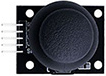
\includegraphics[angle=0, keepaspectratio=true, scale=1, width=200px, height=200px]{images/joystick.jpg}
    %\caption{Caption}
\end{figure}
\subsection*{Description}
The joystick module consists of two potentiometers (one for each axis) and a button. Each axis on the joystick has an analog output associated to it, where the output voltage is directly related to the position of the stick. The josystick can also be clicked but must be debounced.
\subsection*{Pin mapping}
This pin mapping corresponds to the pins from left to right with the module pins facing towards you.
\begin{table}[H]
    \centering
    \begin{tabular}{|c|c|c|c|c|}
    \hline
    Index &Label &Type &Name &Description\\ \hline
    0 &GND &Ground &GND &\\ \hline
    1 &+5V &Source voltage &$V+$ &Module source voltage ($5V$)\\ \hline
    2 &$\text{VR}_\text{x}$ &Analog output &A0 &Joystick x-axis output\\ \hline
    3 &$\text{VR}_\text{y}$ &Analog output &A1 &Joystick y-axis output\\\hline
    4 &SW &Digital output &D0 &Joystick switch output\\ \hline
    \end{tabular}
    %\caption{Caption}
    %\label{tab:my_label}
\end{table}
\subsection*{Operation}
The output voltage at analog pins A0 and A1 depends on the position of the joystick. Moving the joystick on either axis results in either an increase or decrease in the analog output voltage value depending on the direction it was moved. Small fluctuations caused by noise can occur when the joystick is in its resting position, so a dead-zone must be implemented to ensure correct functionality.

Clicking the joystick downwards triggers a button press which sets the digital pin D0 output to low.
\subsection*{Code}
Refer to listing \ref{python_joystick}.
%\lstinputlisting[caption=test]{laser.py} \newpage
\section{Relay module}
\begin{figure}[H]
    \centering
    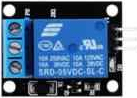
\includegraphics[angle=0, keepaspectratio=true, scale=1, width=200px, height=200px]{images/relay.jpg}
    %\caption{Caption}
\end{figure}
\subsection*{Description}
A DC relay is an electromagnetic switch. Applying a voltage across the relay terminals will close the switch which allows us to control a separate circuit.

\subsection*{Pin mapping}
This pin mapping corresponds to the pins from left to right with the module pins facing towards you.
\begin{table}[H]
    \centering
    \begin{tabular}{|c|c|c|c|c|}
    \hline
    Index &Label &Type &Name &Description\\ \hline
    0 &S &Digital input &D0 &Signal to activate relay \\ \hline
    1 &+ &Source voltage &$V+$ &Module source voltage ($5V$)\\ \hline
    2 &- &Ground &GND &\\ \hline
    \end{tabular}
    %\caption{Caption}
    %\label{tab:my_label}
\end{table}
\subsection*{Operation}
The relay is activated by setting the digital input pin D0 of the module to high. When the relay is activated there will be a short circuit between the NO (Normally open) and COM (Common) terminals. Alternatively, when the relay is not activated there is a short circuit between the NC (Normally closed) and COM (Common) terminals.
%\subsection*{Code}
%\lstinputlisting[caption=test]{laser.py} \newpage
\section{Microphone modules (small \& large)}
\begin{figure}[H]
    \centering
    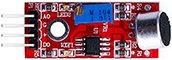
\includegraphics[angle=0, keepaspectratio=true, scale=1, width=200px, height=200px]{images/microphone_large.jpg}
    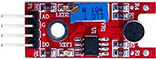
\includegraphics[angle=0, keepaspectratio=true, scale=1, width=200px, height=200px]{images/microphone_small.jpg}
    %\caption{Caption}
\end{figure}
\subsection*{Description}
The microphone modules have both an analog and digital output. When the microphone detects sound the analog output of the module will be proportional to the loudness of the sound. Also if the loudness is above a certain threshold the digital output of the module is set to high.

The microphone is not particularly sensitive, so you may need to blow into the microphone from a close range for it to detect any sound.

\subsection*{Pin mapping}
This pin mapping corresponds to the pins from left to right with the module pins facing towards you.
\begin{table}[H]
    \centering
    \begin{tabular}{|c|c|c|c|c|}
    \hline
    Index &Label &Type &Name &Description\\ \hline
    0 &A0 &Analog output &A0 &Signal to activate relay \\ \hline
    1 &G &Ground &GND &\\ \hline
    2 &+ &Source voltage &$V+$ &Module source voltage ($5V$)\\ \hline
    3 &D0 &Digital output &D0 &\\ \hline
    \end{tabular}
    %\caption{Caption}
    %\label{tab:my_label}
\end{table}
\subsection*{Operation}
The output voltage at the analog pin (A0) is related to the loudness of the sound detected by the microphone.

The output voltage at the digital pin (D0) is set to high when microphone detects a sound louder than a set threshold. This threshold can be set by adjusting the potentiometer on the module.

%\lstinputlisting[caption=test]{laser.py} \newpage

\section{Hall effect sensor (Digital and Analog)}
\begin{figure}[H]
    \centering
    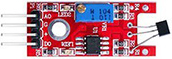
\includegraphics[angle=0, keepaspectratio=true, scale=1, width=200px, height=200px]{images/halleffect_analog_digital.jpg}
    %\caption{Caption}
\end{figure}
\subsection*{Description}
A Hall effect sensor is used to measure the magnitude of a magnetic field near the sensor module. This module has both analog and digital outputs.
\subsection*{Pin mapping}
This pin mapping corresponds to the pins from left to right with the module pins facing towards you.
\begin{table}[H]
    \centering
    \begin{tabular}{|c|c|c|c|c|}
    \hline
    Index &Label &Type &Name &Description\\ \hline
    0 &A0 &Analog output &A0 &\\ \hline
    1 &G &Ground &GND &\\ \hline
    2 &+ &Source voltage &$V+$ &Module source voltage ($5V$)\\ \hline
    3 &D0 &Digital output &D0 &\\ \hline
    \end{tabular}
    %\caption{Caption}
    %\label{tab:my_label}
\end{table}
\subsection*{Operation}
The output voltage at the analog pin (A0) is related to the magnetic field strength near the sensor. When there is no magnetic field, this output is half the supply voltage. As the ESP32 ADC can only measure voltages between 0V to 3.3V, it is recommended to supply the module with 3.3V (for larger swing). Applying a magnetic field oriented in one direction will cause the analog output voltage to be increase, the other direction will cause the voltage to decrease.

The module has a potentiometer to adjust the threshold at which the digital output pin (D0) is set to high.
\subsection*{Code}
Refer to listing \ref{python_hallsensor}.
%\lstinputlisting[caption=test]{laser.py} \newpage
\section{Hall effect sensor (Analog)}
\begin{figure}[H]
    \centering
    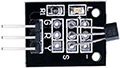
\includegraphics[angle=0, keepaspectratio=true, scale=1, width=200px, height=200px]{images/halleffect_analog.jpg}
    %\caption{Caption}
\end{figure}
\subsection*{Description}
A Hall effect sensor is used to measure the magnitude of a magnetic field near the sensor module. This module has an analog output only.

\subsection*{Pin mapping}
This pin mapping corresponds to the pins from left to right with the module pins facing towards you.
\begin{table}[H]
    \centering
    \begin{tabular}{|c|c|c|c|c|}
    \hline
    Index &Label &Type &Name &Description\\ \hline
    0 &- &Ground &GND &Ground\\ \hline
    1 & &Source voltage &$V+$ &Module source voltage ($3.3V - 5V$)\\ \hline
    2 &S &Analog output &A0 &Hall effect sensor output\\ \hline
    \end{tabular}
    %\caption{Caption}
    %\label{tab:my_label}
\end{table}
\subsection*{Operation}
The output voltage at the analog pin (A0) is related to the magnetic field strength near the sensor. When there is no magnetic field, this output is half the supply voltage. As the ESP32 ADC can only measure voltages between 0V to 3.3V, it is recommended to supply the module with 3.3V (for larger swing). Applying a magnetic field oriented in one direction will cause the analog output voltage to be increase, the other direction will cause the voltage to decrease.
%\subsection*{Code}
%\lstinputlisting[caption=test]{laser.py}
\section{Hall effect sensor (Digital)}
\begin{figure}[H]
    \centering
    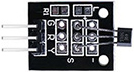
\includegraphics[angle=0, keepaspectratio=true, scale=1, width=200px, height=200px]{images/halleffect_digital.jpg}
    %\caption{Caption}
\end{figure}
\subsection*{Description}
This module is used to detect the prescence of an external magnetic field and has a digital output only.
\subsection*{Pin mapping}
This pin mapping corresponds to the pins from left to right with the module pins facing towards you.
\begin{table}[H]
    \centering
    \begin{tabular}{|c|c|c|c|c|}
    \hline
    Index &Label &Type &Name &Description\\ \hline
    0 &- &Ground &GND &Ground\\ \hline
    1 & &Source voltage &$V+$ &Module source voltage ($3.3V - 5V$)\\ \hline
    2 &S &Digital output &D0 &Hall effect sensor output\\ \hline
    \end{tabular}
    %\caption{Caption}
    %\label{tab:my_label}
\end{table}
\subsection*{Operation}
The digital output pin (D0) is high in the presence of no magnetic field. When a magnetic field is detected D0 is set to low. The sensor can only detect a magnetic field in one direction so try reversing the magnet if the output is not changing.
%\subsection*{Code}
%\lstinputlisting[caption=test]{laser.py} \newpage

\section{Line tracking sensor}
\begin{figure}[H]
    \centering
    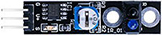
\includegraphics[angle=0, keepaspectratio=true, scale=1, width=200px, height=200px]{images/line_tracking.jpg}
    %\caption{Caption}
\end{figure}
\subsection*{Description}
The line tracking module uses an infrared transmitter and receiver to detect the amount of reflection of the surface in front of it.

The effective distance can range from 2 - 40cm and is adjusted using the potentiometer on the module. A line tracking robot can be implemented using two of these modules (one to check if the robot is drifting left and one to check if the robot is drifting right).

\subsection*{Pin mapping}
This pin mapping corresponds to the pins from left to right with the module pins facing towards you.
\begin{table}[H]
    \centering
    \begin{tabular}{|c|c|c|c|c|}
    \hline
    Index &Label &Type &Name &Description\\ \hline
    0 &G &Ground &GND & \\ \hline
    1 &V+ &Source voltage &$V+$ &Module source voltage ($5V$)\\ \hline
    2 &S &Digital output &D0 &\\ \hline
    \end{tabular}
    %\caption{Caption}
    %\label{tab:my_label}
\end{table}
\subsection*{Operation}
The output voltage at the digital pin (D0) is set to high when the module detects a reflective surface above the set threshold. The circuit is completed when the infrared waves emitted from the transmitter and reflected and absorbed by the infrared receiver.

By adjusting the potentiometer on the module the reflectivity threshold can be changed.
\subsection*{Code}
Refer to listing \ref{python_linetracker}.
%\lstinputlisting[caption=test]{laser.py} \newpage
\section{Obstacle avoidance sensor}
\begin{figure}[H]
    \centering
    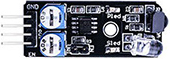
\includegraphics[angle=0, keepaspectratio=true, scale=1, width=200px, height=200px]{images/obstacle_avoidance.jpg}
    %\caption{Caption}
\end{figure}
\subsection*{Description}
The obstacle avoidance sensor works on the same principle as the line tracking sensor module. An infrared transmitter and receiver are placed facing forwards on the module along an on board potentiometer that lets the user adjust the detection range.
\subsection*{Pin mapping}
This pin mapping corresponds to the pins from left to right with the module pins facing towards you.
\begin{table}[H]
    \centering
    \begin{tabular}{|c|c|c|c|c|}
    \hline
    Index &Label &Type &Name &Description\\ \hline
    0 &EN &Unused & &This pin is not used \\ \hline
    1 &VCC &Source voltage &$V+$ &Module source voltage ($5V$)\\ \hline
    2 &OUT &Digital output &D0 &\\ \hline
    3 &GND &Ground &GND &\\ \hline
    \end{tabular}
    %\caption{Caption}
    %\label{tab:my_label}
\end{table}
\subsection*{Operation}
The output voltage at the digital pin (D0) is set to high when the module detects an object. The circuit is completed when the infrared waves emitted from the transmitter and reflected and absorbed by the infrared receiver. As the transmitter and receiver are placed facing forwards on the module, the sensor detects objects in front of the module.

By adjusting the potentiometer on the module the reflectivity threshold can be changed. Note that the potentiometer closest to the ground (GND) pin is factory calibrated and should not be changed.
\subsection*{Code}
Refer to listing \ref{python_avoidance}. \newpage
\section{Flame sensor module}
\begin{figure}[H]
    \centering
    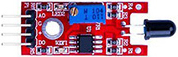
\includegraphics[angle=0, keepaspectratio=true, scale=1, width=200px, height=200px]{images/flame_sensor.jpg}
    %\caption{Caption}
\end{figure}
\subsection*{Description}
The flame sensor module detects infrared light (heat). This module has both analog and digital outputs. The strength of the signal received will depend on the intensity and distance of the flame.
\subsection*{Pin mapping}
This pin mapping corresponds to the pins from left to right with the module pins facing towards you.
\begin{table}[H]
    \centering
    \begin{tabular}{|c|c|c|c|c|}
    \hline
    Index &Label &Type &Name &Description\\ \hline
    0 &A0 &Analog output &A0 &Signal to activate relay \\ \hline
    1 &G &Ground &GND &\\ \hline
    2 &+ &Source voltage &$V+$ &Module source voltage ($5V$)\\ \hline
    3 &D0 &Digital output &D0 &\\ \hline
    \end{tabular}
    %\caption{Caption}
    %\label{tab:my_label}
\end{table}
\subsection*{Operation}
The output voltage pin at the analog pin (A0) is high and decreases towards zero when a flame is detected. A potentiometer on the module allows the adjustment of the sensor threshold. When the sensor reads a value above the threshold the digital pin (D0) is set to high.
\subsection*{Code}
Refer to listing \ref{python_flamesensor}.
%\lstinputlisting[caption=test]{laser.py} \newpage

\section{Touch sensor}
\begin{figure}[H]
    \centering
    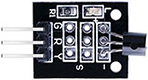
\includegraphics[angle=0, keepaspectratio=true, scale=1, width=200px, height=200px]{images/touch_sensor.jpg}
    %\caption{Caption}
\end{figure}
\subsection*{Description}
This touch sensor module detects changes in capacitances which occur when it is touched by human skin. It has both an analog and digital output but only the digital output is useful.

\subsection*{Pin mapping}
This pin mapping corresponds to the pins from left to right with the module pins facing towards you.
\begin{table}[H]
    \centering
    \begin{tabular}{|c|c|c|c|c|}
    \hline
    Index &Label &Type &Name &Description\\ \hline
    0 &A0 &Analog output &A0 &Unused\\ \hline
    1 &G &Ground &GND &\\ \hline
    2 &+ &Source voltage &$V+$ &Module source voltage ($5V$)\\ \hline
    3 &D0 &Digital output &D0 &\\ \hline
    \end{tabular}
    %\caption{Caption}
    %\label{tab:my_label}
\end{table}
\subsection*{Operation}
The output voltage at the digital pin (D0) is high when the sensor is not being touched and high when the module detects a touch. The on board LED mimics D0 and will turn on when a touch is detected. The potentiometer on the module can be used to adjust sensitivity of the sensor if the LED is on when the sensor is not being touched or if the LED does not turn when the sensor is being touched.
\subsection*{Code}
Refer to listing \ref{python_touchsensor}.
%\lstinputlisting[caption=test]{laser.py} \newpage
\section{Temperature (Digital and Analog)}
\begin{figure}[H]
    \centering
    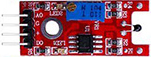
\includegraphics[angle=0, keepaspectratio=true, scale=1, width=200px, height=200px]{images/temperature_digital_analog.jpg}
    %\caption{Caption}
\end{figure}
\subsection*{Description}
A temperature sensor uses a thermistor (a resistor that changes resistance with temperature) and is used to measure the ambient temperature around the module. This module has both analog and digital outputs.
\subsection*{Pin mapping}
This pin mapping corresponds to the pins from left to right with the module pins facing towards you.
\begin{table}[H]
    \centering
    \begin{tabular}{|c|c|c|c|c|}
    \hline
    Index &Label &Type &Name &Description\\ \hline
    0 &A0 &Analog output &A0 &\\ \hline
    1 &G &Ground &GND &\\ \hline
    2 &+ &Source voltage &$V+$ &Module source voltage ($5V$)\\ \hline
    3 &D0 &Digital output &D0 &\\ \hline
    \end{tabular}
    %\caption{Caption}
    %\label{tab:my_label}
\end{table}
\subsection*{Operation}
The output voltage at the analog pin (A0) is related to the ambient temperature around the sensor. Calculating the temperature from the output reading requires some work so refer to the listing associated with this module.
The module has a potentiometer to adjust the threshold at which the digital output pin (D0) is set to high.
%\subsection*{Code}
%\lstinputlisting[caption=test]{laser.py} \newpage
%\include{tex_files/temperaturesensor(digital)} \newpage
\section{Temperature sensor (Analog)}
\begin{figure}[H]
    \centering
    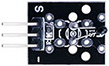
\includegraphics[angle=0, keepaspectratio=true, scale=1, width=200px, height=200px]{images/temperature_analog.jpg}
    %\caption{Caption}
\end{figure}
\subsection*{Description}
A temperature sensor uses a thermistor (a resistor that changes resistance with temperature) and is used to measure the ambient temperature around the module.
\subsection*{Pin mapping}
This pin mapping corresponds to the pins from left to right with the module pins facing towards you.
\begin{table}[H]
    \centering
    \begin{tabular}{|c|c|c|c|c|}
    \hline
    Index &Label &Type &Name &Description\\ \hline
    0 &S &Digital input &D0 &Signal to turn on module\\ \hline
    1 & &Source voltage &$V+$ &Unused\\ \hline
    2 &- &Ground &GND &\\ \hline
    \end{tabular}
    %\caption{Caption}
    %\label{tab:my_label}
\end{table}
\subsection*{Operation}
The output voltage at the analog pin (A0) is related to the ambient temperature around the sensor. Calculating the temperature from the output reading requires some work so refer to the listing associated with this module.
%\subsection*{Code}
%\lstinputlisting[caption=test]{laser.py} \newpage

\section{Active buzzer}
\begin{figure}[H]
    \centering
    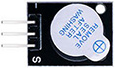
\includegraphics[angle=0, keepaspectratio=true, scale=1, width=200px, height=200px]{images/buzzer1.jpg}
    %\caption{Caption}
\end{figure}
\subsection*{Description}
An active buzzer has an internal oscillator and requires only DC voltage to emit sound. The oscillator turns the input voltage on and off, producing a tone. By using PWM the pitch of the buzzer can be varied.
\subsection*{Pin mapping}
This pin mapping corresponds to the pins from left to right with the module pins facing towards you.
\begin{table}[H]
    \centering
    \begin{tabular}{|c|c|c|c|c|}
    \hline
    Index &Label &Type &Name &Description\\ \hline
    0 &- &Ground &GND &\\ \hline
    1 & &Source voltage &$V+$ &Module source voltage ($5V$)\\ \hline
    2 &S &Analog input &A0 &DC or PWM signal to control buzzer\\ \hline
    \end{tabular}
    %\caption{Caption}
    %\label{tab:my_label}
\end{table}
\subsection*{Operation}
Setting the analog input pin A0 of the buzzer module to high will turn on the buzzer at a constant tone. By applying a PWM signal to A0 the pitch of the buzzer can be varied.
%\subsection*{Code}
%\lstinputlisting[caption=test]{laser.py} \newpage
\section{Passive buzzer}
\begin{figure}[H]
    \centering
    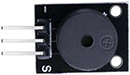
\includegraphics[angle=0, keepaspectratio=true, scale=1, width=200px, height=200px]{images/buzzer2.jpg}
    %\caption{Caption}
\end{figure}
\subsection*{Description}
A passive buzzer has no internal oscillator and requires a PWM signal to operate. By varying the duty cycle and frequency of the PWM signal applied to the passive buzzer the tone and pitch can be varied.
\subsection*{Pin mapping}
This pin mapping corresponds to the pins from left to right with the module pins facing towards you.
\begin{table}[H]
    \centering
    \begin{tabular}{|c|c|c|c|c|}
    \hline
    Index &Label &Type &Name &Description\\ \hline
    0 &- &Ground &GND &\\ \hline
    1 & &Source voltage &$V+$ &Module source voltage ($5V$)\\ \hline
    2 &S &Analog input &A0 &DC or PWM signal to control buzzer\\ \hline
    \end{tabular}
    %\caption{Caption}
    %\label{tab:my_label}
\end{table}
\subsection*{Operation}
Setting the analog input pin A0 of the buzzer module to high will turn on produce no tone. By applying a PWM signal to A0 the tone and pitch of the buzzer can be varied.
\subsection*{Code}
Refer to listing \ref{python_buzzer}.
%\lstinputlisting[caption=test]{laser.py} \newpage

\section{SMT and TH RGB LED modules}
\begin{figure}[H]
    \centering
    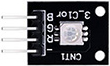
\includegraphics[angle=0, keepaspectratio=true, scale=1, width=200px, height=200px]{images/smd_led.jpg}
    %\caption{Caption}
\end{figure}
\subsection*{Description}
An RGB LED has a pin for each of the three primary colours. The LED module can be controlled by both digital and analog input signals.
\subsection*{Pin mapping}
This pin mapping corresponds to the pins from left to right with the module pins facing towards you.
\begin{table}[H]
    \centering
    \begin{tabular}{|c|c|c|c|c|}
    \hline
    Index &Label &Type &Name &Description\\ \hline
    0 &B &Analog input &A0 &Analog input signal for blue pin \\ \hline
    1 &G &Analog input  &A1 &Analog input signal for green pin \\ \hline
    2 &R &Analog input  &A2 &Analog input signal for red pin \\ \hline
    3 &- &Ground &GND &\\ \hline
    \end{tabular}
    %\caption{Caption}
    %\label{tab:my_label}
\end{table}
\subsection*{Operation}
By applying a PWM signal with varying duty cycle to any of the three pins (A0, A1 and A2) we can control the brightness of each of the three primary colours. Turning multiple colours on at the same time "adds" them together to create other colours.
\subsection*{Code}
Refer to listing \ref{python_rgb}.
%\lstinputlisting[caption=test]{laser.py} \newpage
\section{Two colour LED module}
\begin{figure}[H]
    \centering
    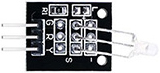
\includegraphics[angle=0, keepaspectratio=true, scale=1, width=200px, height=200px]{images/2_led.jpg}
    %\caption{Caption}
\end{figure}
\subsection*{Description}
This module functions in exactly the same way a regular three colour RGB module, simply with the omission of the blue colour pin. The LED module can be controlled by both digital and analog input signals.
\subsection*{Pin mapping}
This pin mapping corresponds to the pins from left to right with the module pins facing towards you.
\begin{table}[H]
    \centering
    \begin{tabular}{|c|c|c|c|c|}
    \hline
    Index &Label &Type &Name &Description\\ \hline
    0 &- &Ground &GND &\\ \hline
    1 & &Analog input  &A0 &Analog input signal for green pin \\ \hline
    2 &S &Analog input  &A1 &Analog input signal for red pin \\ \hline
    \end{tabular}
    %\caption{Caption}
    %\label{tab:my_label}
\end{table}
\subsection*{Operation}
By applying a PWM signal with varying duty cycle to any of the two pins (A0 and A1) we can control the brightness of each of the two primary colours. Turning both colours on at the same time "adds" them together to create other colours.
\subsection*{Code}
Refer to listing \ref{python_twocoloredled}.
%\lstinputlisting[caption=test]{laser.py} \newpage
\section{Seven colour flashing LED module}
\begin{figure}[H]
    \centering
    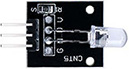
\includegraphics[angle=0, keepaspectratio=true, scale=1, width=200px, height=200px]{images/7_led.jpg}
    %\caption{Caption}
\end{figure}
\subsection*{Description}
This module contains an LED which automatically cycles through seven colours when powered.
\subsection*{Pin mapping}
This pin mapping corresponds to the pins from left to right with the module pins facing towards you.
\begin{table}[H]
    \centering
    \begin{tabular}{|c|c|c|c|c|}
    \hline
    Index &Label &Type &Name &Description\\ \hline
    0 &S &Digital input &D0 &Signal to turn on module\\ \hline
    1 & &Source voltage &$V+$ &Unused\\ \hline
    2 &- &Ground &GND &\\ \hline
    \end{tabular}
    %\caption{Caption}
    %\label{tab:my_label}
\end{table}
\subsection*{Operation}
By setting the digital input pin D0 to high the module can be turned on. Setting D0 to low will turn the module off.
%\subsection*{Code}
%\lstinputlisting[caption=test]{laser.py} \newpage

\section{Reed switch (Digital and Analog)}
\begin{figure}[H]
    \centering
    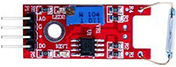
\includegraphics[angle=0, keepaspectratio=true, scale=1, width=200px, height=200px]{images/reed_analog_digital.jpg}
    %\caption{Caption}
\end{figure}
\subsection*{Description}
A reed switch is basically a switch that is activated when a magnetic field is near it.
\subsection*{Pin mapping}
This pin mapping corresponds to the pins from left to right with the module pins facing towards you.
\begin{table}[H]
    \centering
    \begin{tabular}{|c|c|c|c|c|}
    \hline
    Index &Label &Type &Name &Description\\ \hline
    0 &A0 &Analog output &A0 &Unused\\ \hline
    1 &G &Ground &GND &\\ \hline
    2 &+ &Source voltage &$V+$ &Module source voltage ($5V$)\\ \hline
    3 &D0 &Digital output &D0 &\\ \hline
    \end{tabular}
    %\caption{Caption}
    %\label{tab:my_label}
\end{table}
\subsection*{Operation}
The output voltage at the digital output pin (D0) is low when there is an absence of an external magnetic field. When a magnet enters the viscinity of the reed switch the switch is closed and the output of D0 is set to high.

The module has a potentiometer but adjusting will have no noticible effect on the output.
%\subsection*{Code}
%\lstinputlisting[caption=test]{laser.py} \newpage
\section{Mini Reed switch (Digital)}
\begin{figure}[H]
    \centering
    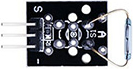
\includegraphics[angle=0, keepaspectratio=true, scale=1, width=200px, height=200px]{images/reed_digital.jpg}
    %\caption{Caption}
\end{figure}
\subsection*{Description}
A reed switch is basically a switch that is activated when a magnetic field is near it. This reed switch is just a simplified version of the above module.
\subsection*{Pin mapping}
This pin mapping corresponds to the pins from left to right with the module pins facing towards you.
\begin{table}[H]
    \centering
    \begin{tabular}{|c|c|c|c|c|}
    \hline
    Index &Label &Type &Name &Description\\ \hline
    0 &S &Digital output &D0 &\\ \hline
    1 & &Source voltage &$V+$ &Module source voltage ($5V$)\\ \hline
    2 &- &Ground &GND &\\ \hline
    \end{tabular}
    %\caption{Caption}
    %\label{tab:my_label}
\end{table}
\subsection*{Operation}
The output voltage at the digital output pin (D0) is low when there is an absence of an external magnetic field. When a magnet enters the vicinity of the reed switch the switch is closed and the output of D0 is set to high.
%\subsection*{Code}
%\lstinputlisting[caption=test]{laser.py} \newpage

%\section{Heartbeat sensor}
\begin{figure}[H]
    \centering
    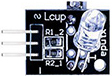
\includegraphics[angle=0, keepaspectratio=true, scale=1, width=200px, height=200px]{images/heartbeat.jpg}
    %\caption{Caption}
\end{figure}
\subsection*{Description}
The heartbeat sensor module consists of an Infrared (IR) LED and a phototransistor (photosensor).
\subsection*{Pin mapping}
This pin mapping corresponds to the pins from left to right with the module pins facing towards you.
\begin{table}[H]
    \centering
    \begin{tabular}{|c|c|c|c|c|}
    \hline
    Index &Label &Type &Name &Description\\ \hline
    0 &S &Analog output &A0 &\\ \hline
    1 & &Source voltage &$V+$ &Module source voltage ($5V$)\\ \hline
    2 &- &Ground &GND &Ground\\ \hline
    \end{tabular}
    %\caption{Caption}
    %\label{tab:my_label}
\end{table}
\subsection*{Operation}
The output voltage at the analog pin (A0) is related to the magnetic field strength near the sensor. When there is no magnetic field, this output is half the supply voltage. As the ESP32 ADC can only measure voltages between 0V to 3.3V, it is recommended to supply the module with 3.3V (for larger swing). Applying a magnetic field oriented in one direction will cause the analog output voltage to be increase, the other direction will cause the voltage to decrease.
\subsection*{Code}
Refer to listing \ref{python_heartbeat}.
%\lstinputlisting[caption=test]{laser.py} \newpage
\section{Laser module}
\begin{figure}[H]
    \centering
    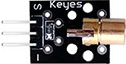
\includegraphics[angle=0, keepaspectratio=true, scale=1, width=200px, height=200px]{images/laser.jpg}
    %\caption{Caption}
\end{figure}
\subsection*{Description}
This module is a red laser pointer.% which creates a small focused dot.
\subsection*{Pin mapping}
This pin mapping corresponds to the pins from left to right with the module pins facing towards you.
\begin{table}[H]
    \centering
    \begin{tabular}{|c|c|c|c|c|}
    \hline
    Index &Label &Type &Name &Description\\ \hline
    0 &S &Digital input &D0 &Signal to turn on module\\ \hline
    1 & &Source voltage &$V+$ &Unused\\ \hline
    2 &- &Ground &GND &\\ \hline
    \end{tabular}
    %\caption{Caption}
    %\label{tab:my_label}
\end{table}
\subsection*{Operation}
By setting the digital input pin D0 to high the module can be turned on. When the module is on a red laser beam will be emitted and a focused red dot can be seen on the surface the laser is pointing at. Setting D0 to low will turn the module off.
\subsection*{Code}
Refer to listing \ref{python_laser}.
%\lstinputlisting[caption=test]{laser.py} \newpage
\section{Tactile switch}
\begin{figure}[H]
    \centering
    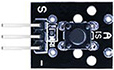
\includegraphics[angle=0, keepaspectratio=true, scale=1, width=200px, height=200px]{images/tactile.jpg}
    %\caption{Caption}
\end{figure}
\subsection*{Description}
This module is a simple tactile switch.
\subsection*{Pin mapping}
A tacticle switch is just a regular button switch.% Pressing the switch will short two sides of the switch and complete the circuit.
\begin{table}[H]
    \centering
    \begin{tabular}{|c|c|c|c|c|}
    \hline
    Index &Label &Type &Name &Description\\ \hline
    0 &S &Digital output &D0 &\\ \hline
    1 & &Source voltage &$V+$ &Unused\\ \hline
    2 &- &Ground &GND &\\ \hline
    \end{tabular}
    %\caption{Caption}
    %\label{tab:my_label}
\end{table}
\subsection*{Operation}
The digital output pin (D0) will be high when the switch is not pressed (open). When the button is pressed and the switch is closed D0 will be set to low.
%\subsection*{Code}
%\lstinputlisting[caption=test]{laser.py} \newpage
\section{Rotary encoder}
\begin{figure}[H]
    \centering
    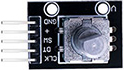
\includegraphics[angle=0, keepaspectratio=true, scale=1, width=200px, height=200px]{images/rotary.jpg}
    %\caption{Caption}
\end{figure}
\subsection*{Description}
This module is different from a potentiometer in that a rotary encoder has full rotation without limits. A rotary encoder module can tell the direction in which it was rotated and by how much.
\subsection*{Pin mapping}
This pin mapping corresponds to the pins from left to right with the module pins facing towards you.
\begin{table}[H]
    \centering
    \begin{tabular}{|c|c|c|c|c|}
    \hline
    Index &Label &Type &Name &Description\\ \hline
    0 &GND &Ground &GND &\\ \hline
    1 &+ &Source voltage &$V+$ &Module source voltage ($5V$)\\ \hline
    2 &SW &Digital input &D0 &Pushbutton switch\\ \hline
    3 &DT & & &Rotary phase B\\ \hline
    4 &CLK & & &Rotary phase A\\ \hline
    \end{tabular}
    %\caption{Caption}
    %\label{tab:my_label}
\end{table}
\subsection*{Operation}
The operation of this module is best explained at \href{https://lastminuteengineers.com/rotary-encoder-arduino-tutorial}{https://lastminuteengineers.com/rotary-encoder-arduino-tutorial}.
\subsection*{Code}
Refer to listing \ref{python_rotaryEncoder}.
%\lstinputlisting[caption=test]{laser.py}we \newpage

\section{Tilt switch}
\begin{figure}[H]
    \centering
    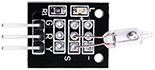
\includegraphics[angle=0, keepaspectratio=true, scale=1, width=200px, height=200px]{images/tilt.jpg}
    %\caption{Caption}
\end{figure}
\subsection*{Description}
This module contains a small amount of conductive liquid in a tube. When the liquid moves to one end of the tube the output voltage is either pulled high or low, and vice versa for the other end. This allows us to monitor if the module is upside down or not.
\subsection*{Pin mapping}
This pin mapping corresponds to the pins from left to right with the module pins facing towards you.
\begin{table}[H]
    \centering
    \begin{tabular}{|c|c|c|c|c|}
    \hline
    Index &Label &Type &Name &Description\\ \hline
    0 &- &Ground &GND &\\ \hline
    1 & &Source voltage &$V+$ &Module source voltage ($5V$)\\ \hline
    2 &S &Digital output &D0 &\\ \hline
    \end{tabular}
    %\caption{Caption}
    %\label{tab:my_label}
\end{table}
\subsection*{Operation}
When the module is upright (not upside down) the voltage of the digital output pin D0 is low. When the module is upside down the voltage of D0 will be set to high.
\subsection*{Code}
Refer to listing \ref{python_tiltswitch}.
%\lstinputlisting[caption=test]{laser.py} \newpage
\section{Ball switch}
\begin{figure}[H]
    \centering
    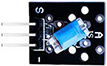
\includegraphics[angle=0, keepaspectratio=true, scale=1, width=200px, height=200px]{images/ball.jpg}
    %\caption{Caption}
\end{figure}
\subsection*{Description}
This module contains a small ball bearing. Operating in a similar fashion to the tilt switch, this module actives when the ball bearing moves to one end of the tube.
\subsection*{Pin mapping}
This pin mapping corresponds to the pins from left to right with the module pins facing towards you.
\begin{table}[H]
    \centering
    \begin{tabular}{|c|c|c|c|c|}
    \hline
    Index &Label &Type &Name &Description\\ \hline
    0 &S &Digital output &D0 &\\ \hline
    1 & &Source voltage &$V+$ &Module source voltage ($5V$)\\ \hline
    2 &- &Ground &GND &\\ \hline
    \end{tabular}
    %\caption{Caption}
    %\label{tab:my_label}
\end{table}
\subsection*{Operation}
When the module is upright the voltage of the digital output pin D0 is low. When the module is in a titled position down the voltage of D0 will be set to high.
\subsection*{Code}
Refer to listing \ref{python_ballswitch}.
%\lstinputlisting[caption=test]{laser.py} \newpage
\section{Shock sensor}
\begin{figure}[H]
    \centering
    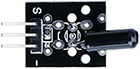
\includegraphics[angle=0, keepaspectratio=true, scale=1, width=200px, height=200px]{images/shock.jpg}
    %\caption{Caption}
\end{figure}
\subsection*{Description}
This module has a very small sensitive spring which absorbs vibrations. The module is triggered when exposed to a shock or a jolt.
\subsection*{Pin mapping}
This pin mapping corresponds to the pins from left to right with the module pins facing towards you.
\begin{table}[H]
    \centering
    \begin{tabular}{|c|c|c|c|c|}
    \hline
    Index &Label &Type &Name &Description\\ \hline
    0 &S &Digital output &D0 &\\ \hline
    1 & &Source voltage &$V+$ &Module source voltage ($5V$)\\ \hline
    2 &- &Ground &GND &\\ \hline
    \end{tabular}
    %\caption{Caption}
    %\label{tab:my_label}
\end{table}
\subsection*{Operation}
When the module is stable the voltage of the digital output pin D0 is low. When the module experiences a shock, jolt or signification vibration the voltage of D0 will be set to high.
\subsection*{Code}
Refer to listing \ref{python_shock}.
%\lstinputlisting[caption=test]{laser.py} \newpage
\section{Vibration sensor}
\begin{figure}[H]
    \centering
    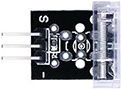
\includegraphics[angle=0, keepaspectratio=true, scale=1, width=200px, height=200px]{images/vibration.jpg}
    \caption{Caption}
\end{figure}
\subsection*{Description}
This module operates on the same principle as the shock sensor and has a very small sensitive spring which absorbs vibrations.
\subsection*{Pin mapping}
This pin mapping corresponds to the pins from left to right with the module pins facing towards you.
\begin{table}[H]
    \centering
    \begin{tabular}{|c|c|c|c|c|}
    \hline
    Index &Label &Type &Name &Description\\ \hline
    0 &S &Digital output &D0 &\\ \hline
    1 & &Source voltage &$V+$ &Module source voltage ($5V$)\\ \hline
    2 &- &Ground &GND &\\ \hline
    \end{tabular}
    %\caption{Caption}
    %\label{tab:my_label}
\end{table}
\subsection*{Operation}
When the module is stable the voltage of the digital output pin D0 is low. When the module experiences signification vibration the voltage of D0 will be set to high.
\subsection*{Code}
Refer to listing \ref{python_vibration}.
%\lstinputlisting[caption=test]{laser.py} \newpage

\section{Photo-resistor}
\begin{figure}[H]
    \centering
    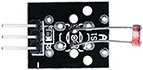
\includegraphics[angle=0, keepaspectratio=true, scale=1, width=200px, height=200px]{images/photosensor.jpg}
    %\caption{Caption}
\end{figure}
\subsection*{Description}
A photo-resistor is a light (brightness) dependant resistor. The photo-resistor is placed in series with a fixed value resistor, creating a voltage divider.

\subsection*{Pin mapping}
This pin mapping corresponds to the pins from left to right with the module pins facing towards you.
\begin{table}[H]
    \centering
    \begin{tabular}{|c|c|c|c|c|}
    \hline
    Index &Label &Type &Name &Description\\ \hline
    0 &S &Analog output &A0 &Photo-resistor output\\ \hline
    1 & &Source voltage &$V+$ &Module source voltage ($5V$)\\ \hline
    2 &- &Ground &GND &Ground\\ \hline
    \end{tabular}
    %\caption{Caption}
    %\label{tab:my_label}
\end{table}
\subsection*{Operation}
When light is shone on the sensor its resistance drops, conversely in low light conditions its resistance remains high (open circuit).

The output voltage at the analog pin (A0) will increase as the brightness or intensity of the light source increases until the photo-resistor acts like a short circuit. When there is no light hitting the sensor module the output at A0 will be zero.
\subsection*{Code}
Refer to listing \ref{python_photoresistor2}.
%\lstinputlisting[caption=test]{laser.py} \newpage
%\include{tex_files/humidty} \newpage
\section{Light blocking (Photo-interrupter) module}
\begin{figure}[H]
    \centering
    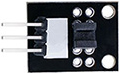
\includegraphics[angle=0, keepaspectratio=true, scale=1, width=200px, height=200px]{images/light_blocking.jpg}
    %\caption{Caption}
\end{figure}
\subsection*{Description}
The photo-interrupter module contains an infrared LED and photo-transistor designed to detect an object in the gap. As the module uses infrared it can detect even transparent objects in the gap.
\subsection*{Pin mapping}
This pin mapping corresponds to the pins from left to right with the module pins facing towards you.
\begin{table}[H]
    \centering
    \begin{tabular}{|c|c|c|c|c|}
    \hline
    Index &Label &Type &Name &Description\\ \hline
    0 &- &Ground &GND &\\ \hline
    1 & &Source voltage &$V+$ &Module source voltage ($5V$)\\ \hline
    2 &S &Analog output &A0 &\\ \hline
    \end{tabular}
    %\caption{Caption}
    %\label{tab:my_label}
\end{table}
\subsection*{Operation}
The output voltage at the analog output pin (A0) is low when the gap is empty. When an object enters the gap the output of A0 will increase until the object has filled the gap at which point the output will be high.
\subsection*{Code}
Refer to listing \ref{python_lightblocking}.
%\lstinputlisting[caption=test]{laser.py} \newpage
\section{Magic light cup module}
\begin{figure}[H]
    \centering
    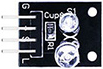
\includegraphics[angle=0, keepaspectratio=true, scale=1, width=200px, height=200px]{images/magic_cup.jpg}
    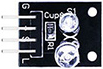
\includegraphics[angle=0, keepaspectratio=true, scale=1, width=200px, height=200px]{images/magic_cup.jpg}
    %\caption{Caption}
\end{figure}
\subsection*{Description}
This module is designed to display an optical effect. The light can 'poured' by tilting the modules as though pouring from one module to the other.

\subsection*{Pin mapping}
This pin mapping corresponds to the pins from left to right with the module pins facing towards you.
\begin{table}[H]
    \centering
    \begin{tabular}{|c|c|c|c|c|}
    \hline
    Index &Label &Type &Name &Description\\ \hline
    0 &G &Ground &GND &\\ \hline
    1 &+ & & &Unused \\ \hline
    2 &S &Digital output &D0 &Output signal from module\\ \hline
    3 &L &Analog input &A0 &Analog signal to module LED\\ \hline
    \end{tabular}
    %\caption{Caption}
    %\label{tab:my_label}
\end{table}
\subsection*{Operation}
The output voltage at the digital pin (D0) is low when the module is upright. When the module is tilted D0 will be set to high.

The LED on the module can be controlled directly setting A0 to high or applying a PWM signal for varying brightness.
%\subsection*{Code}
%\lstinputlisting[caption=test]{laser.py}\newpage

%\DeclareCaptionFormat{}{}

\section*{Code listings}
%\begin{minipage}{\linewidth}\lstinputlisting[label={python_joystick}, caption={Joystick}]{python/joystick.py}\end{minipage}
\lstinputlisting[label={python_joystick}, caption={Joystick}]{python/joystick.py}
\begin{minipage}{\linewidth}\lstinputlisting[label={python_hallsensor}, caption={Hall effect sensor}]{python/hallsensor.py} \end{minipage}
\begin{minipage}{\linewidth}\lstinputlisting[label={python_linetracker}, caption={Line tracking}]{python/linetracker.py}
 \end{minipage}
\begin{minipage}{\linewidth}\lstinputlisting[label={python_avoidance}, caption={Obstacle avoidance}]{python/avoidance.py}
 \end{minipage}
\begin{minipage}{\linewidth}\lstinputlisting[label={python_flamesensor}, caption={Flame sensor}]{python/flamesensor.py}
 \end{minipage}
 \begin{minipage}{\linewidth}\lstinputlisting[label={python_touchsensor}, caption={Flame sensor}]{python/touchsensor.py}
 \end{minipage}
\begin{minipage}{\linewidth}\lstinputlisting[label={python_buzzer}, caption={Passive buzzer}]{python/passiveBuzzer.py}
 \end{minipage}
\begin{minipage}{\linewidth}\lstinputlisting[label={python_rgb}, caption={RGB LEDs}]{python/rgb.py}
 \end{minipage}
\begin{minipage}{\linewidth}\lstinputlisting[label={python_twocoloredled}, caption={2 Coloured LED}]{python/twocolorled.py}
 \end{minipage}
%\begin{minipage}{\linewidth}\lstinputlisting[label={python_heartbeat}, caption={Heartbeat}]{python/heartbeat.py}\end{minipage}
\begin{minipage}{\linewidth}\lstinputlisting[label={python_laser}, caption={Laser}]{python/laser.py}
 \end{minipage}
\begin{minipage}{\linewidth}\lstinputlisting[label={python_rotaryEncoder}, caption={Rotary encoder}]{python/rotaryEncoder.py}
 \end{minipage}
\begin{minipage}{\linewidth}\lstinputlisting[label={python_tiltswitch}, caption={Tilt switch}]{python/tiltswitch.py}
 \end{minipage}
\begin{minipage}{\linewidth}\lstinputlisting[label={python_ballswitch}, caption={Ball switch}]{python/ballswitch.py}
 \end{minipage}
\begin{minipage}{\linewidth}\lstinputlisting[label={python_shock}, caption={Shock sensor}]{python/shock.py}
 \end{minipage}
\begin{minipage}{\linewidth}\lstinputlisting[label={python_vibration}, caption={Vibration sensor}]{python/vibration.py}
 \end{minipage}
\begin{minipage}{\linewidth}\lstinputlisting[label={python_photoresistor2}, caption={Photo-resistor}]{python/photoresistor2.py}
 \end{minipage}
\begin{minipage}{\linewidth}\lstinputlisting[label={python_lightblocking}, caption={Light blocking}]{python/lightblocking.py} \end{minipage}
%\lstinputlisting[label={python_avoidance}, caption={test}]{python/shock.py}

\end{document}
